%==============================================================================
\chapter{Ergebnisse} \label{chap:ergebnis}
%==============================================================================

In diesem Kapitel werden mit der vorgeschlagenen Modellierung von Kraftstoffsystemen für Fluggasturbinen berechnete Ergebnisse analysiert. Dabei steht insbesondere die Frage im Fokus, ob die Modellierung den Leistungs- und Wärmebedarf der Kraftstoffsysteme akkurat vorhersagen kann. Zunächst wird eine Sensitivitäts-Analyse durchgeführt, um die Auswirkung der in Kapitel \  Danach wird die Methodik dieser Arbeit daher mit Daten aus der Literatur validiert. Anschließend wird im Rahmen einer Parameterstudie analysiert, wie sich die Eintrittstemperaturen des Kraftstoffs in den Wärmeübertrager und die Brennkammer auf die Modellierungen der Wasserstoff-Kraftstoffsysteme auswirkt. Abschließend erfolgt ein Vergleich des Betriebsmittelbedarfs der Wasserstoff-Kraftstoffsysteme untereinander und mit dem Referenzkraftstoffsystem anhand eines ausgewählten Betriebspunkts.

\section{Validierung}

Zur Validierung der Methodik dieser Arbeit wird das Wasserstoff-Kraftstoffsystem mit Pumpe angepasst und parametriert, um das von Brewer \cite{Brewer.1991} vorgeschlagene Kraftstoffsystem nachzuempfinden. 

Dabei werden folgende Modifikationen an der Modellierung vorgenommen: Die Druckverluste im rezirkulierten Kraftstoffstrom werden vernachlässigt, da das Kraftstoffsystem nach Brewer keinen Rezirkulationsverdichter vorsieht. Der Kraftstoffmassenstrom wird nicht an die Brennkammer-Eintrittstemperatur und Leistungsentnahmen angepasst und eine parallele Wasserstoffverbrennung ist nicht vorgesehen. Zudem bleibt der Wärmeeintrag des von Brewer vorgeschlagenen Rekuperators unberücksichtigt, da sich dieser Wärmeübertrager Stromabwärts der Entnahmestelle des rezirkulierten Kraftstoffs befindet - eine Konfiguration, die von der Modellierung dieser Arbeit abweicht. Um dennoch eine Vergleichbarkeit der Pumpenleistung zu gewährleisten, wird der Druckverlust dieses Wärmeübertragers zu den Druckverluste der Injektoren addiert. 

Ein weiterer Unterschied liegt in der Modellierung des Kraftstoffs: Während in dieser Arbeit Parawasserstoff verwendet wird, basieren Brewers Berechnungen auf Normalwasserstoff. Dies macht eine Anpassung der Modellparameter des Wasserstoff-Stoffmodels erforderlich. Tabelle \ref{Tab:brewer} zeigt die weiteren Änderungen der Parameter und Variablen gegenüber dem ursprünglichen Wasserstoff-Kraftstoffsystem mit Pumpe.

\begin{table}[ht]
    \centering
	\caption{Veränderte Parameter der Validierung}
	\begin{tabular} {|l|c|c|c|} \hline%
    \multicolumn{2}{|c|}{Parameter} & Einheit & Wert\\ \hline\hline%
    FOHE Druckverhältnis & $\pi_\mathrm{FOHE}$ & - & 1 \\ \hline
    Brennkammer-Massenstrom & $\dot{m}_\mathrm{BK}$ & kg/s & 0,166 \\ \hline
    Leitungsdruckverluste & $\Delta p_\mathrm{r}$ & kPa & 30 \\ \hline
    Injektordruckverluste & $\Delta p_\mathrm{inj}$ & kPa & 214,4 \\ \hline
    Brennkammer-Eintrittsdruck & $p_\mathrm{BK}$ & kPa & 1516,2 \\ \hline
    Brennkammer-Eintrittstemperatur & $T_\mathrm{BK}$ & K & 264 \\ \hline
    Wärmeübertrager-Eintrittstemperatur & $T_\mathrm{W}$ & K & 200 \\ \hline
    \end{tabular}	
    \label{Tab:brewer}%
\end{table}
\FloatBarrier 

Tabelle \ref{Tab:validation} zeigt die von Brewer berechneten Werte und die mit der beschriebenen Methodik berechneten Werte. 

\begin{table}[ht]
    \centering
	\caption{Validierung der Methodik}
	\begin{tabular} {|l|c|c|c|c|} \hline%
    \multicolumn{2}{|c|}{Variable} & Einheit & Brewer \cite{Brewer.1991} & Diese Arbeit \\ \hline\hline%
    Pumpenleistung & $P_\mathrm{HPFP}$ & kW & 23,9 & 23,4 \\ \hline
    Wärme & $\dot{Q}$ & kW & 542,7 & 539,8 \\ \hline
    Rezirkulierter Massenstrom & $\dot{m}_\mathrm{R}$ & kg/s & 0,377 & 0,439 \\ \hline
    Pumpen-Austrittstemperatur & $T_{2,\mathrm{HPFP}}$ & K & 50 & 33,1 \\ \hline
    \end{tabular}	
    \label{Tab:validation}%
\end{table}
\FloatBarrier 

Die Werte für die Pumpenleistung und den Wärmebedarf stimmen weitgehend mit den Berechnungen von Brewer überein. Allerdings berechnet Brewers einen um $14\,\%$ geringeren rezirkulierten Massenstrom, was auf die um \SI{16.9}{\K} höhere Pumpen-Austrittstemperatur mit seinem Modell zurückzuführen ist. Um den Ursprung dieser Abweichung zu identifizieren, wird die Energiebilanz verwendet. Die Energiebilanz um die Hochdruckpumpe des Brewer-Konzepts 

\begin{equation}\label{Eq:brewer}
	\Delta \dot{E}_\mathrm{HPFP}=\dot{m}_\mathrm{BK}(h(T_0,p_0)-h(T_\mathrm{HPFP}, p_\mathrm{HPFP}))+P_\mathrm{HPFP}
\end{equation}

weist ein Residuum von $\Delta \dot{E}_\mathrm{HPFP}=$ \SI{-79.9}{\kilo\W} auf. Ähnliche Energiebilanzen für die Wasserstoffmischung und die Wärmeübertrager ergeben Residuen von $\Delta \dot{E}_\mathrm{mix}=$ \SI{25.3}{\kilo\W} und $\Delta \dot{E}_\mathrm{W}=$ \SI{57.2}{\kilo\W}. Da das Residuum der Energiebilanz des gesamten Kraftstoffsystems mit $\Delta \dot{E}=$ \SI{2.3}{\kilo\W} gering ist, erscheint ein Fehlerursprung im verwendeten Stoffmodell als unwahrscheinlich. Die Abweichungen auf Komponenten-Ebene könnten durch einen nicht dokumentierten Wärmeübertrager zwischen flüssigem und verdampften Wasserstoff erklärt werden. Aufgrund dieser Problematik ist eine belastbare Validierung der Methodik dieser Arbeit nicht möglich.

\section{Parameterstudie}

Um die Wechselwirkung zwischen Wärmeübertrager- und Brennkammer-Eintritts-temperatur auf die Betriebsmittelbedarfe der Wasserstoff-Kraftstoffsysteme zu untersuchen wird eine zweidimensionale Parameterstudie durchgeführt. Die Parameter und Konfiguration der Wasserstoff-Kraftstoffsysteme werden über den untersuchten Bereich als konstant angenommen. Da sich die Wasserstoff-Kraftstoffsysteme untereinander in ihrem Verhalten weitgehend ähneln, werden die Ergebnisse zunächst für die Architektur mit Hochdruckpumpe gezeigt. Anschließend werden die Unterschiede zwischen den Architekturen im Detail betrachtet.

\subsection{Architektur mit Hochdruckpumpe}

Abbildung \ref{fig:pumppower} zeigt den mechanischen Leistungsbedarf des Wasserstoff-Kraftstoffsystems mit Pumpe für den untersuchten Temperaturbereich. 

\begin{figure}[ht]
\centering
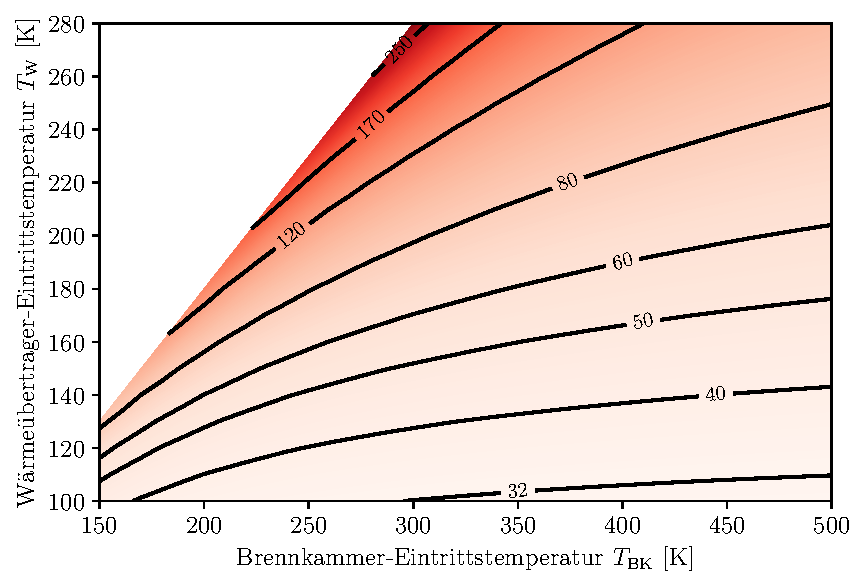
\includegraphics[width=0.9\linewidth]{4_Abbildungen/2_Hauptteil/Ergebnisse/Pumpepowercontour.pdf}
  \caption{Leistungsbedarf Wasserstoff-Kraftstoffsystem mit Pumpe [kW]}
  \label{fig:pumppower}
\end{figure}
\FloatBarrier

Der Gesamtleistungsbedarf steigt mit zunehmender Wärmeübertrager-Eintrittstemperatur, da die geringe Differenz zur Brennkammer-Eintrittstemperatur eine verstärkte Kraftstoffrezirkulation erfordert, was die Leistung des Rezirkulationsverdichters erhöht. Zwar führen höhere Brennkammer-Eintrittstemperaturen zu einer Zunahme der spezifischen Arbeit des Rezirkulationsverdichters, jedoch wird dieser Effekt durch den aufgrund der erhöhten Temperaturdifferenz reduzierten rezirkulierten Massenstrom mehr als ausgeglichen. Die Leistung der Hochdruckpumpe ist hingegen unabhängig von den Eintrittstemperaturen (Abbildung \ref{fig:pumpsplit}). 

\begin{figure}[ht]
\centering
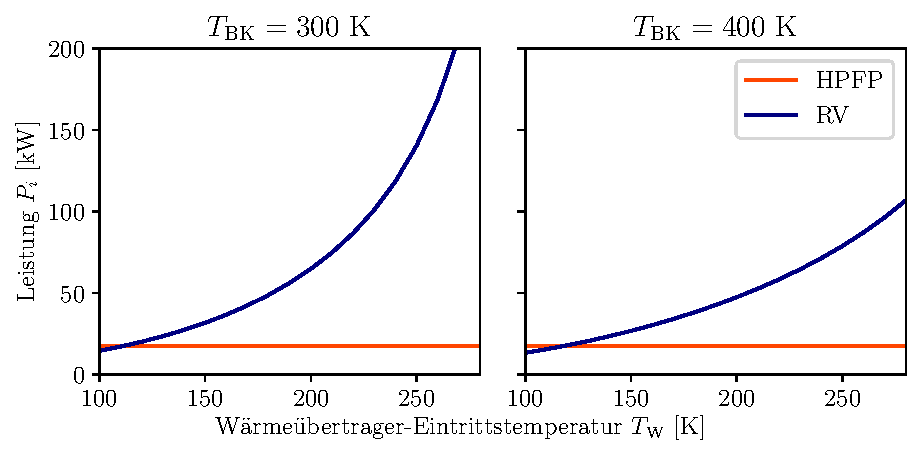
\includegraphics[width=0.9\linewidth]{4_Abbildungen/2_Hauptteil/Ergebnisse/Pumpe_powersplit.pdf}
  \caption{Leistungsaufteilung Architektur mit Pumpe}
  \label{fig:pumpsplit}
\end{figure}
\FloatBarrier

Der Wärmebedarf ist insbesondere mit der Brennkammer-Eintrittstemperatur korreliert. Da die Leistung des Rezirkulationsverdichters mit steigender Wärmeübertrager-Eintrittstemperatur beziehungsweise geringer Differenz der Eintrittstemperaturen zunimmt, liegt in diesem Fall ein verringerter Wärmebedarf vor. Dieses Verhalten ist in Abbildung \ref{fig:pumpheat} dargestellt.

\begin{figure}[ht]
\centering
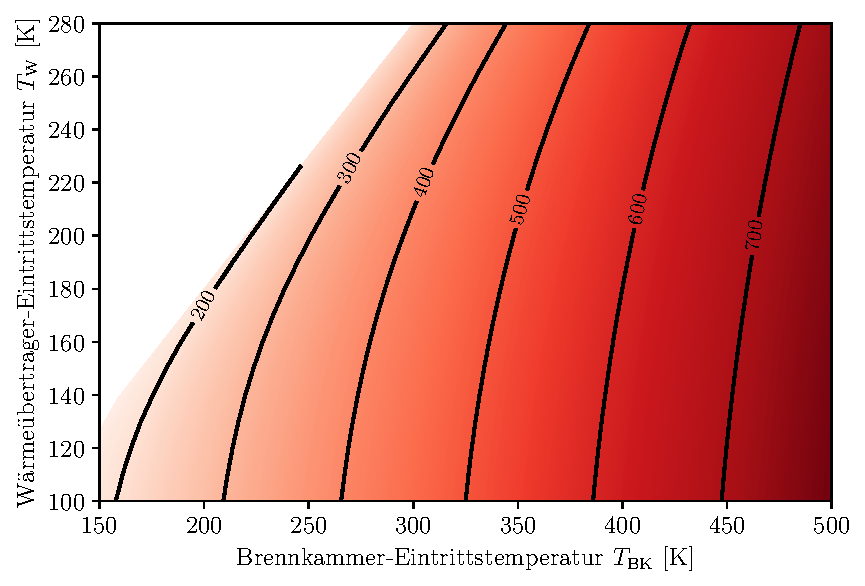
\includegraphics[width=0.9\linewidth]{4_Abbildungen/2_Hauptteil/Ergebnisse/Pumpeheatcontour.pdf}
  \caption{Wärmebedarf Wasserstoff-Kraftstoffsystem mit Pumpe [kW]}
  \label{fig:pumpheat}
\end{figure}
\FloatBarrier

Abbildung \ref{fig:pumpfuel} zeigt den Kraftstoffverbrauch des Triebwerks mit dem Kraftstoffsystem mit Pumpe für die unterschiedlichen Eintrittstemperaturen.

\begin{figure}[ht]
\centering
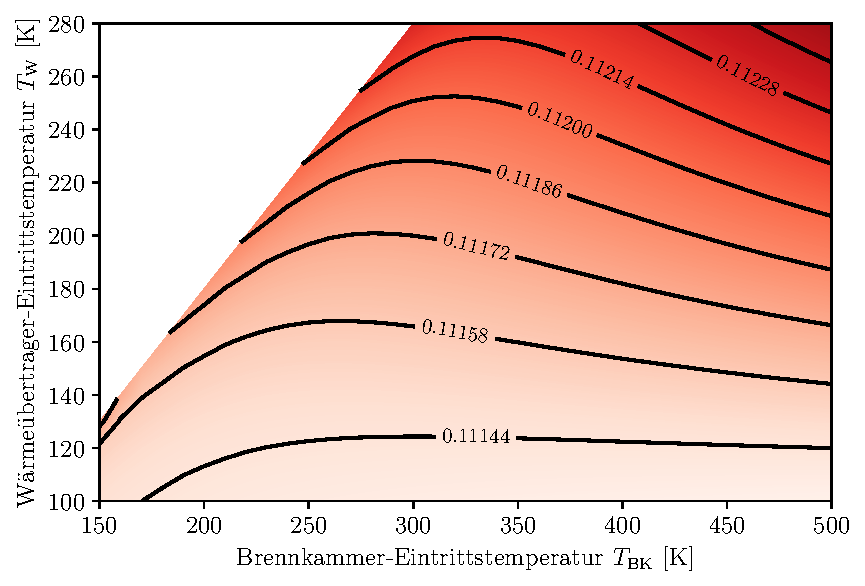
\includegraphics[width=0.9\linewidth]{4_Abbildungen/2_Hauptteil/Ergebnisse/Pumpemassflowcontour.pdf}
  \caption{Kraftstoffverbrauch Wasserstoff-Kraftstoffsystem mit Pumpe [kg/s]}
  \label{fig:pumpfuel}
\end{figure}
\FloatBarrier

Die Leistung des Rezirkulationsverdichters bei hohen Wärmeübertrager-Eintritts-temperaturen verringert den Gesamtwirkungsgrad des Triebwerks. Im Gegensatz dazu hat die Brennkammer-Eintrittstemperatur einen geringeren Einfluss auf den Verbrauch.


\subsection{Vergleich der Wasserstoff-Kraftstoffsysteme}

Im Folgenden werden die Ergebnisse der Parameterstudie für die verschiedenen Wasserstoff-Kraftstoffsysteme miteinander verglichen. Abbildung \ref{fig:comp_power} zeigt den Leistungsbedarf der Kraftstoffsysteme in Abhängigkeit der Wärmeübertrager-Eintrittstemperatur für zwei verschiedene Brennkammer-Eintrittstemperaturen.

\begin{figure}[ht]
\centering
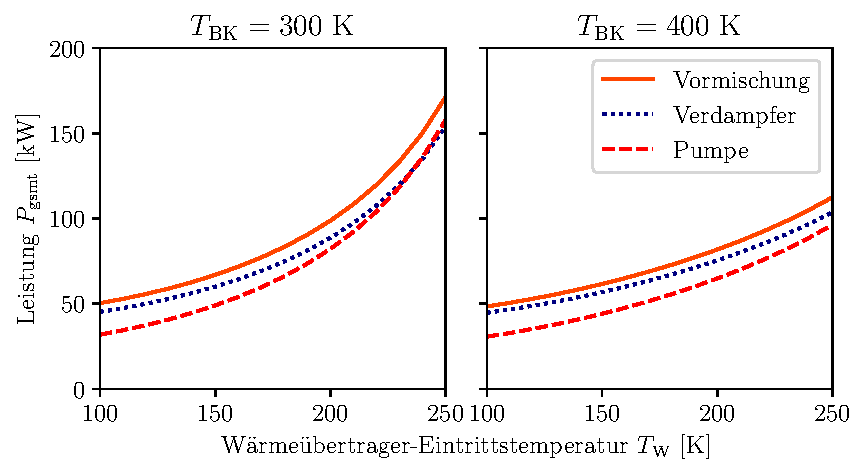
\includegraphics[width=0.9\linewidth]{4_Abbildungen/2_Hauptteil/Ergebnisse/summary_power.pdf}
  \caption{Leistungsbedarf Wasserstoff-Kraftstoffsysteme}
  \label{fig:comp_power}
\end{figure}
\FloatBarrier

Aufgrund der höheren spezifischen Arbeit der Verdichtung im gasförmigen Zustand weisen beide Verdichterarchitekturen im Vergleich zur Pumpenarchitektur einen erhöhten Leistungsbedarf auf. Da die Verdichter des Kraftstoffsystems mit Vormischung bei identischer spezifischer Arbeit einen größeren Massenstrom  fördern als die Verdichter der Architektur mit Verdampfer, hat das Kraftstoffsystem mit Vormischung einen höheren Leistungsbedarf. Dieser Effekt wird bei höheren Brennkammer-Eintrittstemperaturen abgeschwächt, da die Verdampfung in diesem Fall einen geringeren Massenstrom erfordert. Abbildung \ref{fig:comp_split} zeigt den Einfluss der Wärmeübertrager-Eintrittstemperatur auf die Komponenten-Leistungen.

\begin{figure}[ht]
\centering
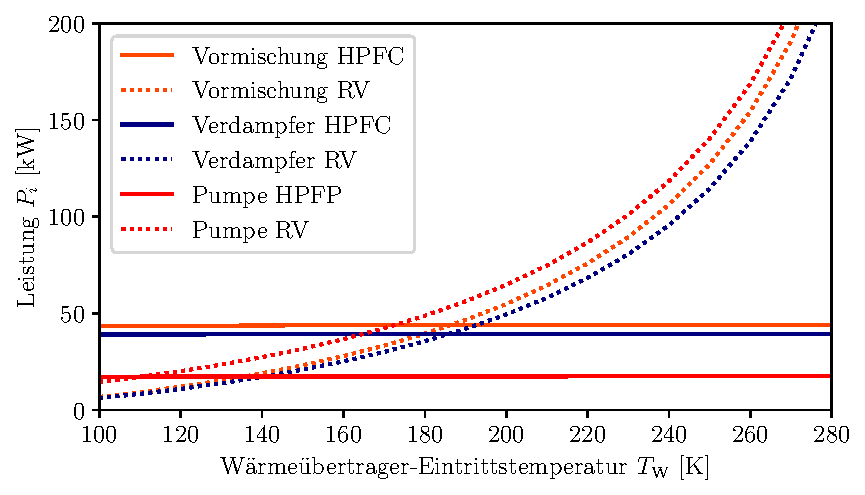
\includegraphics[width=0.9\linewidth]{4_Abbildungen/2_Hauptteil/Ergebnisse/300summary_powersplit.pdf}
  \caption{Leistungsaufteilung Vergleich [$T_\mathrm{BK}=$ \SI{300}{\K}]}
  \label{fig:comp_split}
\end{figure}
\FloatBarrier

Analog zur Architektur mit Pumpe hat die Wärmeübertrager-Eintrittstemperatur bei den Verdichterarchitekturen keinen Einfluss auf die Leistung des Hochdruckverdichters. Da die Verdichterarchitekturen im Vergleich zur Pumpenarchitektur einen geringeren Rezirkulationsmassenstrom aufweisen, fällt auch die Leistung des Rezirkulationsverdichters geringer aus. Abbildung \ref{fig:tbk_split} zeigt den Einfluss der Brennkammer-Eintrittstemperatur auf die Komponenten-Leistungen.

\begin{figure}[ht]
\centering
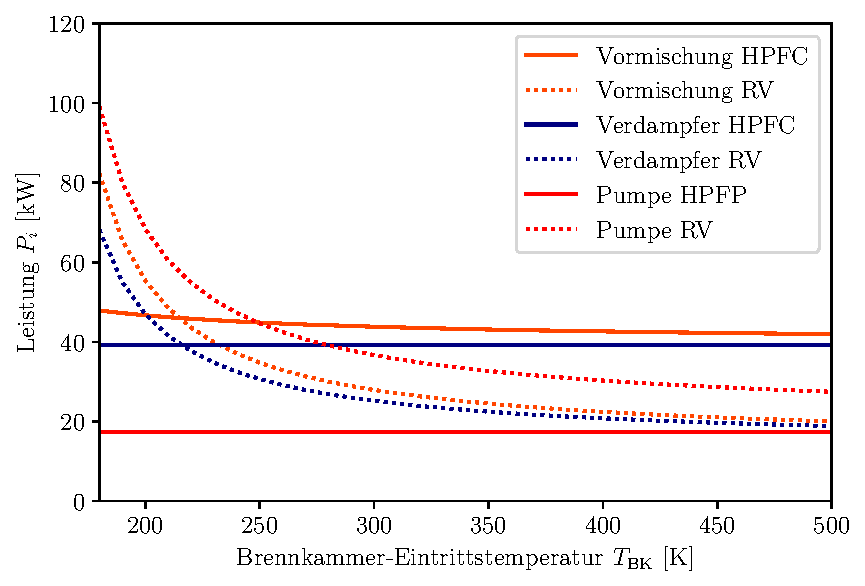
\includegraphics[width=0.7\linewidth]{4_Abbildungen/2_Hauptteil/Ergebnisse/tbkcomp.pdf}
  \caption{Leistungsaufteilung Vergleich [$T_\mathrm{W}=$ \SI{160}{\K}]}
  \label{fig:tbk_split}
\end{figure}
\FloatBarrier

Der Trend sinkender Leistung des Rezirkulationsverdichters bei höherer Differenz der Eintrittstemperaturen setzt sich auch bei den Verdichterarchitekturen fort. Im Gegensatz zu den anderen Architekturen führen steigende Brennkammer-Eintrittstemperaturen bei der Architektur mit Vormischung jedoch zu einer geringfügigen Reduzierung der Leistung des Hochdruckverdichters. Dies ist auf den geringeren erforderlichen Massenstrom für die Verdampfung zurückzuführen. 

Abbildung \ref{fig:stackplot} gibt einen Überblick der Leistungsanteile der Wasserstoff-Kraftstoffsysteme. In der linken Spalte sind die Leistungsanteile in Abhängigkeit der Brennkammereintritts-Temperatur bei konstanter Wärmeübertrager-Eintrittstemperatur dargestellt. Die mittlere Spalte zeigt die Leistungsanteile in Abhängigkeit der Brennkammer-Eintrittstemperatur, aber mit konstanter Temperaturdifferenz. Die rechte Spalte zeigt die Leistungsanteile in Abhängigkeit der Wärmeübertrager-Temperatur bei konstanter Brennkammereintritts-Eintrittstemperatur.

\begin{figure}[ht]
\centering
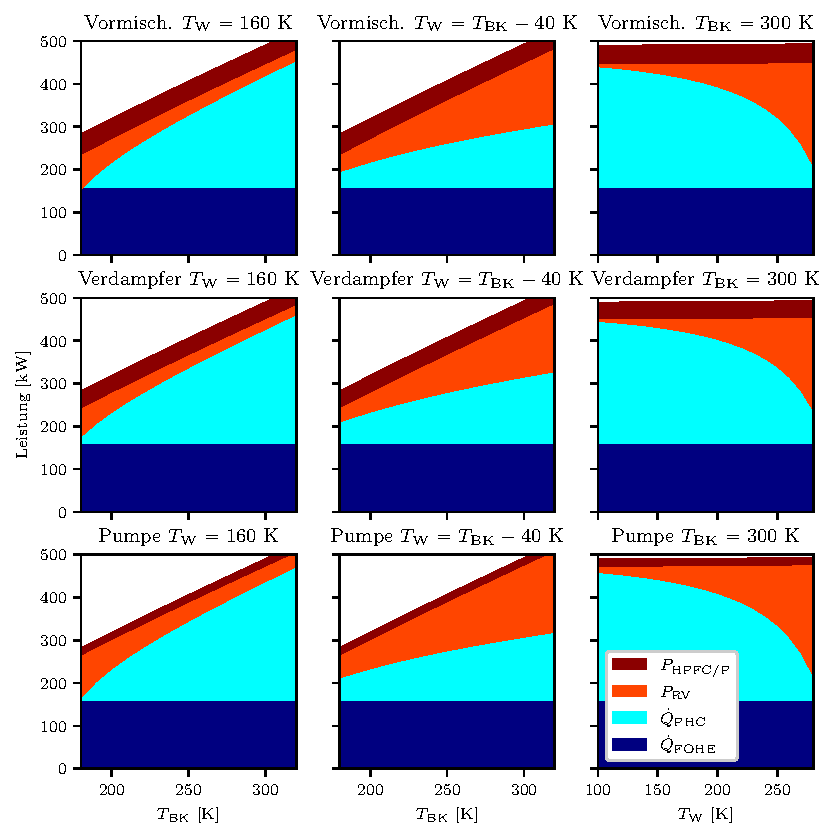
\includegraphics[width=1\linewidth]{4_Abbildungen/2_Hauptteil/Ergebnisse/stackplot_summary.pdf}
  \caption{Stapeldiagramme der Leistungsanteile}
  \label{fig:stackplot}
\end{figure}
\FloatBarrier

Diese Abbildung verdeutlicht den Einfluss der Differenz der Eintrittstemperaturen. Bei einer konstanten Temperaturdifferenz von $T_{BK}-T_W=$ \SI{40}{\K} (mittlere Spalte) liegen die Leistung des Rezirkulationsverdichters $P_{RV}$ und die Wärme der parallelen Wasserstoffverbrennung $\dot{Q}_{PHC}$ über die untersuchten Brennkammer-Eintrittstemperaturen betragsmäßig in einem ähnlichen Bereich. Im Gegensatz dazu nimmt bei konstanter Brennkammer-Eintrittstemperatur der Leistungsanteil des Rezirkulationsverdichters mit steigender Wärmeübertrager-Eintrittstemperatur zu (rechte Spalte).

Eine direkte Empfehlung spezifischer Eintrittstemperaturen lässt sich aus diesen Daten nicht ableiten. Grundsätzlich gilt, dass eine möglichst niedrige hinnehmbare Wärmeübertrager-Eintrittstemperatur den Kraftstoffverbrauch reduziert. Für die Brennkammer-Eintrittstemperatur lässt sich hingegen keine eindeutige Aussage treffen, sodass sie in Abhängigkeit von der Wärmeübertrager-Eintrittstemperatur gewählt werden sollte.

\section{Vergleich mit dem Referenzmodell}

Im Folgenden werden die Wasserstoff-Kraftstoffsysteme mit dem Referenzkraftstoffsystem verglichen. Abbildung \ref{fig:refcomp} zeigt den Betriebsmittelbedarf der verschiedenen Kraftstoffsysteme. Für die Wasserstoff-Kraftstoffsysteme gilt eine Brennkammer-Eintrittstemperatur von $T_\mathrm{BK}=$ \SI{300}{\K} und eine Wärmeübertrager-Eintrittstemperatur von $T_\mathrm{W}=$ \SI{160}{\K}.

\begin{figure}[ht]
\centering
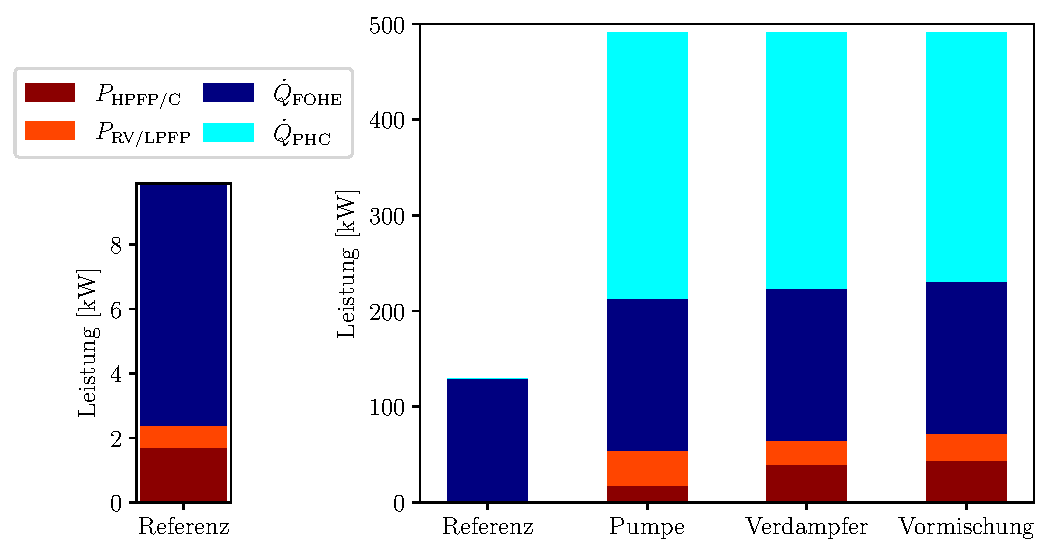
\includegraphics[width=1\linewidth]{4_Abbildungen/2_Hauptteil/Ergebnisse/refcomp.pdf}
  \caption{Betriebsmittelbedarf der Kraftstoffsysteme}
  \label{fig:refcomp}
\end{figure}
\FloatBarrier

Der Betriebsmittelbedarf der Wasserstoff-Kraftstoffsysteme übersteigt den Bedarf des Referenzkraftstoffsystems um einen Faktor von drei. Im Vergleich zum Referenzkraftstoffsystem erfordert das Wasserstoff-Kraftstoffsystem mit Pumpe 22,7-Mal mehr Leistungsentnahme von der Hochdruckwelle und hat einen Wärmefehlbetrag von \SI{278}{\kilo\W}, der durch die parallele Wasserstoffverbrennung gedeckt wird. Bei dem Kraftstoffsystem mit Verdampfer wird sogar das 27,1-Fache an Leistungsentnahme benötigt bei einem Wärmefehlbetrag von \SI{268}{\kilo\W}. Bei dem Kraftstoffsystem mit Vormischung wird das 30,2-Fache an Leistungsentnahme benötigt bei einem Wärmefehlbetrag von nur noch \SI{261}{\kilo\W}. 

Um die Vergleichbarkeit des Kraftstoffverbrauchs sicherzustellen, wird der Energieverbrauch als Produkt aus dem Kraftstoffverbrauch und dem unteren Heizwert bei Normaldruck und einer Temperatur von \SI{298.15}{\K} berechnet.
Abbildung \ref{fig:refenergy} zeigt die Differenz des Energieverbrauchs der Wasserstoff-Kraftstoffsysteme zum Referenzkraftstoffsystem. 

\begin{figure}[ht]
\centering
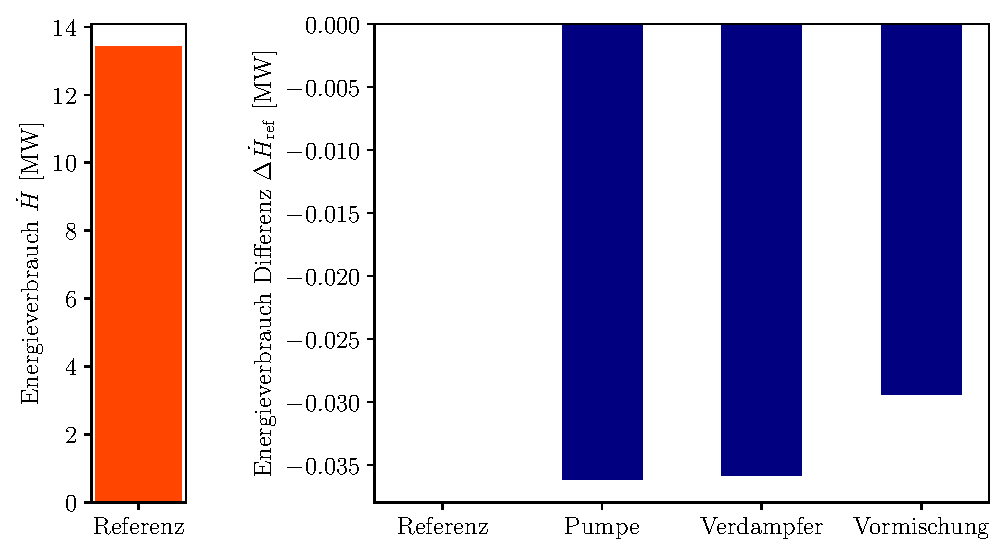
\includegraphics[width=1\linewidth]{4_Abbildungen/2_Hauptteil/Ergebnisse/refenergy.pdf}
  \caption{Energieverbrauch der Kraftstoffsysteme}
  \label{fig:refenergy}
\end{figure}
\FloatBarrier

Trotz des zusätzlichen Betriebsmittelbedarfs verbrauchen die Wasserstoff-Kraftstoffsysteme bis zu $0{,}27\,\%$ weniger Energie. Dies ist auf den höheren Wirkungsgrad des Kreisprozesses des wasserstoffbetriebenen Zyklus zurückzuführen, der durch die abweichenden Abgaseigenschaften begünstigt wird.